\chapter{Preliminaries and Dataset}\label{chap:method}

\section{Preliminaries}

\subsection{RDF, Ontology, and SPARQL}
The Resource Description Framework (RDF)is a framework to represent data in the web~\cite{rdf_framework}. It is an XML based language to represent the information that is present on the web. RDF contains basic three elements: Property, Resource, and Statement (subject, predicate, and object). For example a statement ``Stuti knows Tom Hanks'' would translate to \texttt{uri://people\#StutiNayak25 http://xmlns.com/foaf/0.1/knows uri://people\#TomHanks62}. 

W3C defines an ontology as “the terms used to describe and represent an area of
knowledge”~\cite{heflin2004owl}. An ontology defines a common vocabulary for researchers who need to share information in a domain. It includes machine-interpretable definitions of basic concepts in the domain and relations among them~\cite{noy2001ontology}. Everyone has their own definitions when it comes to ontology, another definition given by~\cite{gruber1993translation,gruber1995toward} - ``from an AI point of view, an ontology is defined as the \emph{explicit specification of organization}'' which is widely accepted in the AI community. It is further explained that an ontology should be considered as an agreement regarding \emph{shared conceptualizations}. Shared conceptualizations include conceptual frameworks for modeling domain knowledge; content-specific protocols for communication among inter-operating agents; and agreements about the representation of particular domain theories. In the knowledge sharing context, ontologies are specified in the form of definitions of representational vocabulary. A very simple case would be a type hierarchy, specifying classes and their subsumption relationships.

Lastly, when we want to extract information that we want using the RDF data we need a query language there we use SPARQL~\cite{harris2013sparql}. It can also be used to manipulate data stored in RDF format. It supports various result formats namely: the Extensible Markup Language (XML), the JavaScript Object Notation (JSON), Comma Separated Values (CSV), and Tab Separated Values (TSV). 




%%%%%%%%%%%%%%%%%%%%%%%%%%%%%%%%%%%%%%%%%%%%%%%%%%%%%%%%%%%%%%%%%%%%%%%%%%%%%%%%%%%%%%%%%%%%%%%%%%%%%%%
%\subsection{Neural Networks}
%The neural network approach is widely used in machine learning and deep learning algorithms to solve problems with complex, sparse data~\cite{lecun2015deep}. In a neural network architecture, there are layers which are classified into three types which are mentioned below, all these layers contain nodes which are interconnected to each other in a dense manner also shown in Figure~\ref{fig:nn}:
%\begin{itemize}
   % \item \textbf{input layer} - this brings in the data into the architecture which is then passed on to the next layer for processing
   % \item \textbf{hidden layer(s)} - after the input layers there are a certain number of interconnected layers these can be specified accordingly. Here, the network takes a bunch of weighted sets and use an activation function to emit the output.
    %\item \textbf{output layer} - the last layer of nodes where we get the output.
%\end{itemize}

%    \begin{figure}[ht]       \centering
 %       \includegraphics[scale=0.3]{Figures/Neural_network.png}
  %      \caption{A simple neural network architecture}
  %      \label{fig:nn}
  %  \end{figure}

%\paragraph{Multilayer Perceptrons} or short for MLPs is one of the classical forms of a neural network. This can be used for solving regression problems or classification problems or datasets in the form of a table.  


%\paragraph{Convolutional Neural Newtorks} short for CNN are widely used when dealing with image data~\cite{krizhevsky2012imagenet}. One of the reasons why they are successful in image data because of its property of keeping a number of copies of the same type of neurons. This helps the model to have numerous neurons while being able to process large complex models keeping the same number of parameters. While writing programs in computer science we tend to write a function and keep calling it, later on, the CNNs do a similar thing with the help of these large number of neurons. This, in turn, makes learning easier and reduces error. 

%The CNNs also have three types of layers: (i) Convolutional Layers, (ii) Pooling Layers and (iii) Fully-Connected Layers. The convolutional layers are the feature maps which are downsampled by the pooling layers. The fully-connected layers are towards the end to compute probabilities of the outputs.
%%%%%%%%%%%%%%%%%%%%%%%%%%%%%%%%%%%%%%%%%%%%%%%%%%%%%%%%%%%%%%%%%%%%%%%%%%%%%%



\section{Dataset}\label{section:data}
As mentioned earlier in Chapter~\ref{chap:intro} for re-using we need to understand the metadata. 
An example of a GEO sample is shown in the Figure~\ref{figure: sample}. 
\begin{figure}[h!]
\centering
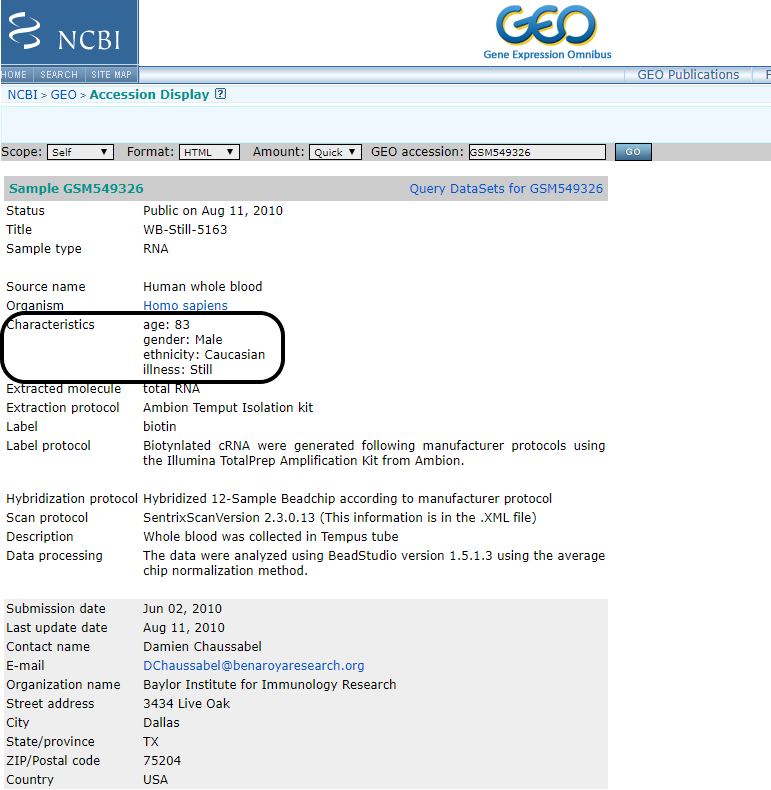
\includegraphics[scale=0.5]{Figures/sample.png}
\caption{An example of GEO Sample}
\label{figure: sample}
\end{figure}
The highlighted part is the field characteristics. The field is structured as key: value pairs where ``age'' is the key and the number $83$ is the value. We chose the ``characteristics'' field since it is semi-structured.
Examples of good metadata and bad metadata in presented in Figure~\ref{fig:bad_meadata} and~\ref{fig:biosample}. From the Figure~\ref{fig:bad_meadata}, in the field about gender it is filled with the number $2$ - which is semantically inaccurate as it is unclear what the 2 refers to. Thus it is difficult to understand what that Sample was about. Similarly, there is no way a human being lives for 160 years, but in the metadata \emph{age: 160} is mentioned. If someone wants to understand what this information is about except that it is something about human beings, it would not be a very trivial task. On the other hand, from the Figure~\ref{fig:biosample}, one can make out the experiments involved human beings and about leukemia.

\begin{figure}[ht]
    \centering
    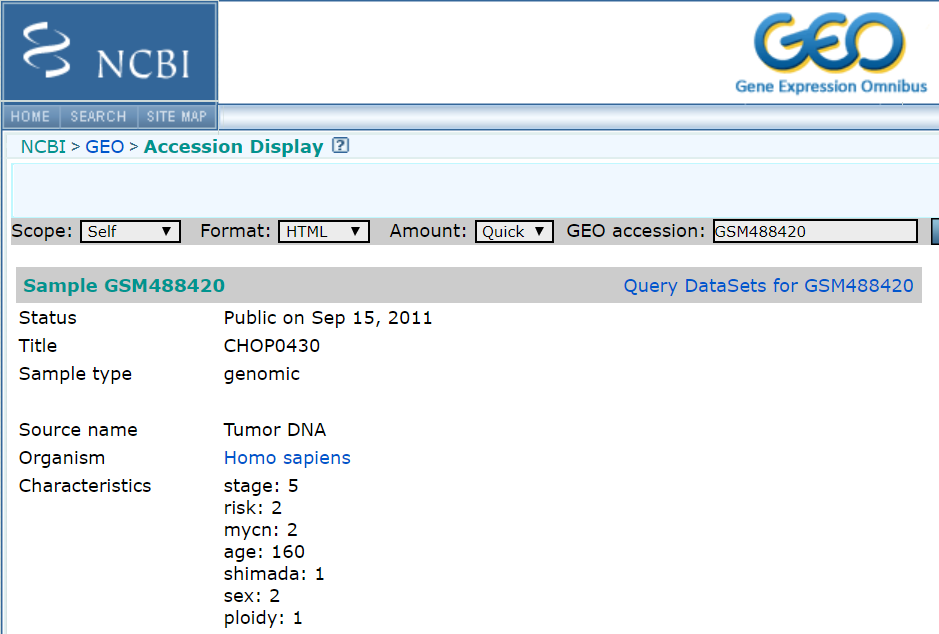
\includegraphics[scale=0.5]{Figures/Capture_geo.png}
    \caption{Example of a bad metadata}
    \label{fig:bad_meadata}
\end{figure}

\begin{figure}[ht]
    \centering
    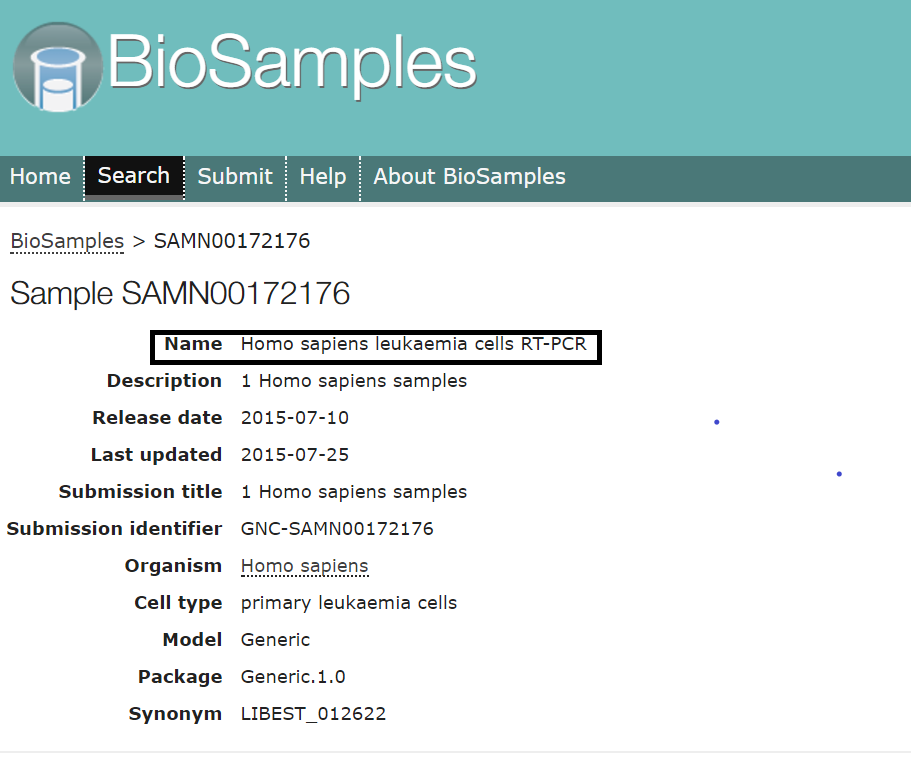
\includegraphics[scale = 0.4]{Figures/Biosamples.png}
    \caption{Example of a satisfactory metadata}
    \label{fig:biosample}
\end{figure}

%\todo{write more about why this dataset and why disease}
The scientific publications contain a lot of information about the experiments done, this information would be useful to determine good metadata. Therefore for predicting metadata, the first step is to look for a gold standard dataset which would have annotated terms of metadata elements. We first start with the metadata category \emph{disease}, for that we need to have a dictionary which can be used for predicting disease values. Therefore, for this purpose, we use the NCBI Disease Corpus~\cite{dougan2014ncbi}. This corpus identifies disease terms using 14 human annotators in 793 scientific publication abstracts and titles from PubMed~\footnote{\url{https://www.ncbi.nlm.nih.gov/pubmed/}}, which serves the purpose as when we test the model with a known scientific text we would know how accurate are the predictions. This corpus identifies disease terms and links it to ontology namely Medical Subject Headings (MeSH)\footnote{\url{https://www.nlm.nih.gov/mesh/}} and Online Mendelian Inheritance in Man (OMIM)\footnote{\url{https://www.omim.org/}}. 

The disease names identified are classified into the following four concepts: 
\begin{itemize}
    \item DiseaseClass: A string which represents a family of diseases, then it was annotated to a disease class. For example: ``autosomal recessive disease'' is a \emph{Disease Class} category.  
    
    \item SpecificDisease: A string that does not have any children class. For example: ``Diastrophic dysplasia'' is a \emph{Specific Disease}. 
    
    \item Modifier: A string that is a disease name but it might modify a sentence containing a noun. In simple words, if a disease name occurs which is a secondary and tries to focus on any other disease is annotated as a \emph{Modifier}. 
    
    For example: In the abstract text ``Although this mutation was initially detected in four of 33 colorectal cancer families analysed from eastern England, more extensive analysis has reduced the frequency to four of 52 English HNPCC kindreds analysed.'' 
    
    The experts are asked to annotate in this way: ``colorectal cancer'' as Modifier category and ``HNPCC'' as Modifier category. 
    
    \item CompositeMention: If more than one disease names occur together then that string was annotated to \emph{Composite Mention}. 
    
    For example, a protein required for ubiquitin-mediated degradation of beta-catenin, but a small percentage of colon and some other cancers harbour beta-catenin-stabilizing mutations. 
    
    The Annotation is - ``colon and some other cancers'': CompositeMention
    
\end{itemize}
 An example of annotation is shown in Listing~\ref{annotation}. 
The number $10192393$ is the PubMed Identifier, the string ``$|$t$|$'' denotes the title and ``$|$a$|$'' denotes the abstract of the scientific publications. All the terms below the abstract are the identified disease terms such as skin tumour, cancer etc. The terms ``D012878'', ``D009369'' are the unique identification number of skin tumour and cancer respectively from the MeSH ontology. 

\begin{lstlisting}[caption=An example of annotation, label=annotation]
10192393|t|A common human skin tumour is caused by activating mutations in beta-catenin.
10192393|a|WNT signaling orchestrates a number of developmental programs. In response to this stimulus, cytoplasmic beta-catenin (encoded by CTNNB1) is stabilized, enabling downstream transcriptional activation by members of the LEF/TCF family. One of the target genes for beta-catenin/TCF encodes c-MYC, explaining why constitutive activation of the WNT pathway can lead to cancer, particularly in the colon. Most colon cancers arise from mutations in the gene encoding adenomatous polyposis coli (APC), a protein required for ubiquitin-mediated degradation of beta-catenin, but a small percentage of colon and some other cancers harbour beta-catenin-stabilizing mutations. Recently, we discovered that transgenic mice expressing an activated beta-catenin are predisposed to developing skin tumours resembling pilomatricomas... 
10192393    15    26    skin tumour    DiseaseClass    D012878
10192393    443    449    cancer    DiseaseClass    D009369
10192393    483    496    colon cancers    DiseaseClass    D003110
10192393    539    565    adenomatous polyposis coli    SpecificDisease    D011125
10192393    567    570    APC    SpecificDisease    D011125

\end{lstlisting}

As mentioned earlier, the corpus contains in total 793 PubMed titles and abstracts which is divided into three sets (i) training, (ii) testing and (iii) development. The Table~\ref{table_ncbi} shows details of the corpus:

\begin{table}[h!]
\caption{NCBI disease Corpus characteristics}
\label{table_ncbi}
\begin{tabular}{|c|c|c|c|}
\hline
\textbf{Corpus Characteristics} & \textbf{Training} & \textbf{Development} & \textbf{Testing} \\ \hline
PubMed Citations                & 593               & 100                  & 100              \\ \hline
Disease Mentions                & 5,148             & 791                  & 961              \\ \hline
Specific Disease                & 2,959             & 409                  & 556              \\ \hline
Disease Class                   & 781               & 127                  & 121              \\ \hline
Modifier                        & 1,292             & 218                  & 264              \\ \hline
Composite Mention               & 116               & 37                   & 20               \\ \hline
\end{tabular}
\end{table}

%As mentioned in Table~\ref{table_ncbi} the corpus contains 793, the Figure shows a word cloud of the abstract text.
The corpus is annotated by fourteen domain experts. There were two-annotators per document which were paired randomly. The annotation was completed in three phases and was checked for consistency throughout the whole corpus as shown in the Figure~\ref{fig:annotationdetails}. In total, we have $2136$ diseases. The statistics of the annotations are as follows are shown in Table~\ref{table: input_stats}. 

\begin{figure}[ht]
    \centering
    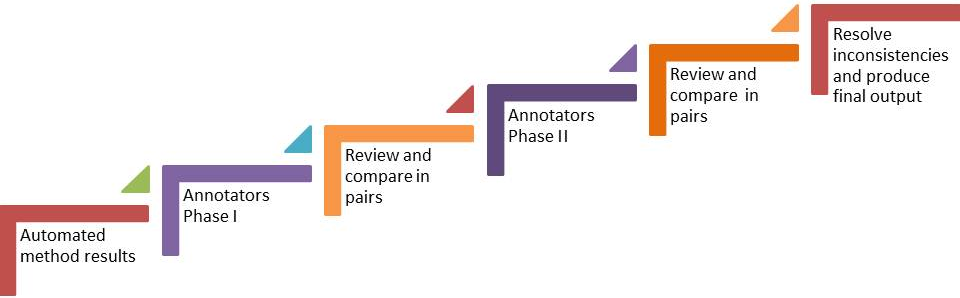
\includegraphics[scale=0.5]{Figures/annotationprocess.png}
    \caption{Annotation Process (Source: \url{https://www.ncbi.nlm.nih.gov/CBBresearch/Dogan/DISEASE/})}
    \label{fig:annotationdetails}
\end{figure}

\begin{table}[ht]
\caption{Input corpus statistics}
\label{table: input_stats}
\centering
\begin{tabular}{|l|l|}
\hline
\textbf{Target Labels} & \textbf{Count} \\ \hline
CompositeMention       & 112            \\ \hline
DiseaseClass           & 571            \\ \hline
Modifer                & 222            \\ \hline
SpecificDisease        & 1231           \\ \hline
\textbf{Grand Total}   & \textbf{2136}  \\ \hline
\end{tabular}
\end{table}


\paragraph{Data Preprocessing}
In the dataset, we have a set of scientific publication titles and abstracts in addition to the identified disease terms and respective disease concepts from the ontology as we saw in the Listing~\ref{annotation}. 
Since a neural network model cannot process raw text data, there is a need to perform some preprocessing stops.
Firstly, the data is cleaned by removing all the (i) punctuation (filters=\verb|’!”#$%&()*+,-./:;<=>?@[\\]^_|), (ii) numbers and (iii) convert all the text into lowercase.  
For training the model, we only use (i) the abstract, (ii) the disease names and (iii) the Unique ID of these diseases from the MeSH ontology. The abstract is used because it contains more information when compared to the title. After that, the text is separated from the disease names as we treat the disease names as the labels that would be identified using the text by the model.
We get the following characteristics of the abstracts:
\begin{itemize}
    \item max length:  450
    \item mean:  191.1640826873385
    \item min length:  32
    \item median:  190.0
\end{itemize}
\paragraph{Text Preprocessing} The text is tokenized - converted into a list of words, and fit according to the size of the text, this converts the text into a set of words which could be called tokens.
Then these tokens are integer encoded - given a unique index, the highest number being the size of the words. 
Then we convert these words into a sequence which gives the words a unique identification number. Then we need to pad this sequence which means to normalize the sequences into a maximum length so that the neural network knows what length of the sequence to expect. 
For example - some sentences will be less than 200 let's say 155, so we insert 45 zeros to make it 200. Some might be bigger say 220, so we remove last 20. We test the model with varying sequence lengths. 

%\paragraph{Label Matrix} To construct a label matrix we need to create a one-hot encoded matrix of the size of the labels we have. In this context, the labels are disease names, for example, if we have 3 diseases the encoded vectors would be in the form of the Table~\ref{table:one_hot}. 

%\begin{table}[ht]
%\caption{Example of one-hot encoding}
%\label{table:one_hot}
%\centering
%\begin{tabular}{|c|c|c|}
%\hline
%\multicolumn{1}{|l|}{disease1} & \multicolumn{1}{l|}{disease2} & \multicolumn{1}{l|}{disease 3} \\ \hline
%1                              & 0                             & 0                         %     \\ \hline
%0                              & 1                             & 0                         %     \\ \hline
%0                              & 0                             & 1                         %     \\ \hline
%\end{tabular}
%\end{table}


%\subsection{Feature Selection}
%For feature selection a Term frequency-inverse document (TF-IDF) approach is used. For each document, a weight is assigned to each term which is essentially the number of times that term occurs in the document (i.e. the frequency of the term.)

%\section{Neural Network Method}
%Chapter~\ref{chap:nnmethod}
